\documentclass[11pt,letterpaper]{article}

\usepackage[utf8]{inputenc}
\usepackage{amsmath,amsthm,amssymb}
\usepackage{fullpage}
\usepackage[ruled]{algorithm2e}
\usepackage{tikz}
\usepackage{esvect}
\usepackage{caption}
\usepackage{subcaption}
\usepackage[left= 3 cm,right=3 cm,top=3 cm,bottom=3 cm]{geometry}
\usepackage{mathtools}
\usepackage[colorlinks = true, citecolor = {blue}]{hyperref}
\usepackage{array}
\usepackage{comment}
\usepackage{authblk}

\newtheorem{theorem}{Theorem}
\newtheorem{lemma}{Lemma}
\newtheorem{corollary}{Corollary}
\newtheorem{definition}{Definition}

%%%%%% COMMANDS %%%%%%
\newcommand{\defoptproblem}[3]{
 \vspace{1mm}
\noindent\fbox{
 \begin{minipage}{0.96\textwidth}
 #1 \\
 {\bf{Input:}} #2 \\
 {\bf{Output:}} #3
 \end{minipage}
 }
 \vspace{1mm}
}


\newcommand{\set}[1]{\left\{ #1 \right\}}
\newcommand{\card}[1]{\left| #1 \right|}
\newcommand{\ith}[1]{#1^{\mbox{\scriptsize{th}}}}

% algo
\newcommand{\checkperp}{\mbox{\textsf{check}}^{\perp}}
\newcommand{\ifend}{\textbf{endif}}

%diam - radius - ecc
\newcommand{\diam}{\mbox{\textsf{diam}}}
\newcommand{\rad}{\mbox{\textsf{rad}}}
\newcommand{\ecc}{\mbox{\textsf{ecc}}}
\newcommand{\wecc}[2]{\mbox{\textsf{ecc}}\left(#1 ~\vert ~ #2\right)}
\newcommand{\opp}{\mbox{\textsf{op}}}
\newcommand{\rc}{\mbox{RC}}
\newcommand{\paradj}{\parallel_{\mbox{\scriptsize{P}}}}
\newcommand{\paradjc}{\parallel_{\scriptsize{\Theta}}}
\newcommand{\paradji}{\parallel_{\scriptsize{\Theta}}^{-1}}
\newcommand{\perpadj}{\perp_{\scriptsize{\Theta}}}
\newcommand{\paradjm}{\parallel_{\mbox{\scriptsize{Pm}}}}
\newcommand{\ulog}{\mathcal{U}_{2\log}}
\newcommand{\med}{\mbox{Med}}
\newcommand{\umax}{u_{\max}}


%% comments %%
\newcommand{\PB}[1]{{\color{orange} Pierre: #1}}

\title{Quasilinear time for computing all eccentricities of median graphs}

\author[1]{Pierre Berg\'e Chaikovskaia}
\author[2,3]{Guillaume Ducoffe}
\author[4]{Michel Habib}
%Beaudou Bergé Dailly Gérard Lagoutte Limouzy Pastor
\affil[1]{Université Clermont-Auvergne, CNRS, Mines de Saint-Etienne,
	Clermont-Auvergne-INP, LIMOS, 63000 Clermont-Ferrand, France}
\affil[2]{National Institute for Research and Development in Informatics, Romania}
\affil[3]{University of Bucharest, Romania}
\affil[4]{IRIF, CNRS, Universit\'e Paris Cité, France}

\date{}

\begin{document}

\maketitle

\begin{abstract}
\textbf{Contributions}:
\begin{itemize}
    \item Compute all eccentricities of median graphs in quasilinear time
    \item Oracle for finding distances in $O(\sqrt{n})$
    \item Distance profile for diameter-bounded median graphs ?
\end{itemize}
\textbf{Directions of research}:
\begin{itemize}
    \item Distance labeling scheme of polylogarithmic size
\end{itemize}
\end{abstract}

\bigskip

\section{Introduction} \label{sec:intro}

\defoptproblem{\textsc{Eccentricities}}{A median graph $G = (V,E)$.}{All labels $\wecc{u}{G} = \max \{d(u,v) : v \in V\}$ for each vertex $u \in V$.}

\defoptproblem{\textsc{Weighted Eccentricities}}{A weighted median graph $G = (V,E,\omega)$, with $\omega : V \rightarrow \mathbb{N}$.}{All labels $\wecc{u}{(G,\omega)} = \max \{d(u,v) + \omega(v) : v \in V\}$ for each $u \in V$.}

\section{Preliminaries} \label{sec:notation}

We begin with a reminder of some notions of graphs, and more particularly related to median graphs. We emphasize on a very important tool in this area: $\Theta$-classes, which are equivalences classes over the edge set, and especially the orthogonality between two $\Theta$-classes.

\subsection{Graph properties} 

All graphs $G = (V,E)$ considered in this paper are undirected, simple, finite and connected. To avoid confusions when several graphs are considered, we denote by $V(G)$ (resp. $E(G)$) the vertex set (resp. edge set) of $G$. Let $N(u)$ be the \textit{open neighborhood} of $u \in V$, {\em i.e.} the set of vertices adjacent to $u$ in $G$. We extend it naturally: for any set $A \subseteq V$, the neighborhood $N(A)$ of $A$ is the set of vertices outside $A$ adjacent to some $u \in A$.

A subgraph $G'$ of $G$ is a graph $G'=(V',E')$, where $V' \subseteq V$ and $E' \subseteq E\cap (V' \times V')$. 
%In this case, we use the notation $G' \subseteq G$. 
For any $U \subseteq V$, we denote by $E\left[U\right]$ the set of edges of $G$ with two endpoints in $U$. We denote by $G\left[U\right]$ the subgraph of $G$ induced by $U$: $G\left[U\right] = \left(U,E\left[U\right]\right)$. 
%We denote by $G\setminus U$ the graph deprived of vertices in $U$: $G\setminus U = G\left[V\setminus U\right]$. Similarly, for any set of edges $E' \subseteq E$, the graph $G$ deprived of $E'$ is denoted by $G\setminus E' = \left(V,E\setminus E',\omega_{|E \setminus E'}\right)$.

Given two vertices $u,v \in V$, let $d(u,v)$ be the \textit{distance} between $u$ and $v$, {\em i.e.} the length of the shortest $(u,v)$-path. The \textit{eccentricity} $\ecc(u)$ of a vertex $u \in V$ is the length of the longest shortest path starting from $u$. Put formally, $\ecc(u)$ is the maximum value $d(u,v)$ for all $v \in V$: $\ecc(u) = \max_{v \in V} d(u,v)$. When the context is not clear enough, we might notice, as a subscript, in which graph these distance are considered, {\em e.g.} $d_G(u,v)$, $\ecc_G(u)$. The diameter of graph $G$ is the maximum distance between two of its vertices: $\diam(G) = \max_{u \in V} \ecc_G(u)$. 

We denote by $I(u,v)$ the \textit{interval} of pair $u,v$. It contains exactly the vertices which are metrically between $u$ and $v$:
$I(u,v) = \set{x \in V: d(u,x) + d(x,v) = d(u,v)}$. The vertices of $I(u,v)$ are lying on at least one shortest $(u,v)$-path.

\begin{definition}[Convex and gated sets]
We say that a set $H\subseteq V$ (or the induced subgraph $G\left[H\right]$) is \emph{convex} if $I(u,v) \subseteq H$ for any pair $u,v \in H$. Moreover, we say that $H$ is \emph{gated} if any vertex $v \notin H$ admits a $H$-\emph{gate} $g_H(v) \in H$, {\em i.e.} a unique vertex that belongs to all intervals $I(v,x)$, $x\in H$. For any $x \in H$, we have $d(v,g_H(v)) + d(g_H(v),x) = d(v,x)$. 
\end{definition}

Gated sets are convex by definition. Indeed, by contradiction, for a gated set $H$, if a shortest path from $x\in H$ to $y\in H$ was containing a section outside $H$, it would imply the existence of two $H$-gates for the vertices of this section. Conversely, convex sets are not necessarily gated in general ({\em e.g.} any pair of vertices in the $K_3$). But, we will see in the remainder that it is true on median graphs. A well-known property is that the intersection of two gated sets is itself gated.

\begin{lemma}[Intersection of gated subgraphs~\cite{BaCh08}]
Given two gated sets $H_1,H_2$ of a graph $G$, the set $H_1\cap H_2$ is gated. 
\label{le:intersection}
\end{lemma}

We naturally focus on the set of vertices which admit a given vertex as a gate.

\begin{definition}[Fibers]
Given a gated set $H$ of $G$ and a vertex $x \in H$, the \textit{fiber} $F_H[x]$ is the set of vertices which admit $x \in H$ as a gate for $H$. As each vertex in $H$ is its own gate, the fibers $F_H[x]$, $x \in H$ form a partition of $V(G)$.
\end{definition}

A fiber is thus a set of vertices which all admit the same gate for a given $H$. Observe that, except $x$ itself, $F_H[x]$ contains vertices outside $H$: $F_H[x] \setminus \{x\} \subseteq V(G) \setminus H$. In the following sections, we often manipulate this set $F_H[x] \setminus \{x\}$ that we call the \emph{open fiber}.

\begin{definition}[Open fibers]
Given a gated set $H$ of $G$ and a vertex $x \in H$, we define the \emph{open fiber} as $F_H(x) = F_H[x] \setminus \{x\}$.
\label{def:open_fiber}
\end{definition}

There is a natural linear-time algorithm (in fact, a very slight variation of BFS) for computing the fibers (and open fibers) of a given gated set $H$. To keep this paper as self-contained as possible, we recall a sketch of this algorithm, proposed in~\cite{ChLaRa19}. The classical BFS uses a queue to store the visited vertices of the graph. Here, we initialize this queue by putting into it all the vertices of $H$ (instead of a single starting vertex). Each vertex $v \in V$ is labeled by three variables: $d(v)$ (distance to the gate), $f(v)$ (parent of $v$ in the BFS tree) and $\texttt{fib}(v)$ ($H$-gate of $v$). All vertices $x \in H$ are initialized with $d(x) = 0$, $f(x) = \texttt{NULL}$, and $\texttt{fib}(x) = x$. 
Then, we proceed the search as follows. Once a vertex $v$ is at the head of the queue, all not yet discovered neighbors $w$ of $v$ are inserted into the queue, and we fix $d(w) = d(v) + 1$, $f(w) = v$, $\texttt{fib}(w) = \texttt{fib}(v)$. At the end of the execution, each vertex $v$ is labeled by its gate $\texttt{fib}(v) = g_H(v)$ in $H$. For the correctness of this BFS traversal, see Lemma 16 and Corollary 6 from~\cite{ChLaRa18}, the open access version of~\cite{ChLaRa19}.

\begin{lemma}[\cite{ChLaRa18,ChLaRa19}]
For any gated set $H$ of a graph $G$, one can compute all fibers $F_H(x)$, with $x\in H$, in linear time $O(m)$.
\label{le:compute_gates}
\end{lemma}

In this article, we say a \textit{weighted graph} is a generalization $(G,\omega)=(V,E,\omega)$ where the vertices are labeled with nonnegative integer weights: $\omega : V \rightarrow \mathbb{N}$. Observe that the definitions of the structural notions above are independent from any weight consideration.

Now, considering a weighted graph $(G,\omega)$, the distance is naturally generalized to a \textit{weighted distance} which is not symmetrical anymore: $d_{\omega}(u,v) = d(u,v) + \omega(v)$. When there is some ambiguity on the graph considered, we may write this weighted distance $d_{(G,\omega)}(u,v)$. The \textit{weighted eccentricity} of a vertex $u \in V$ is the maximum weighted distance from this vertex, {\em i.e.} $\wecc{u}{(G,\omega)} = \max_{v \in V} d_{\omega}(u,v)$. 

However, notions of interval, gate, convex and gated sets, fiber remain independent from the weight function $\omega$. Their definition is only based on the unweighted distance.

\subsection{Median graphs and $\Theta$-classes}

From now on, we focus on the family of graphs which is studied in this article: median graphs. 

\begin{definition}[Median graph]
A graph is \textit{median} if, for any triplet $x,y,z$ of distinct vertices, the set $I(x,y) \cap I(y,z) \cap I(z,x)$ contains exactly one vertex $m(x,y,z)$ called the median of $x,y,z$.
\label{def:median}
\end{definition}

Observe that certain well-known families of graphs are median: trees, grids, squaregraphs~\cite{BaChEp10}, and hypercubes $Q_k$.
Median graphs are bipartite and do not contain an induced $K_{2,3}$~\cite{BaCh08,HaImKl11,Mu78}. They can be obtained by Mulder's convex expansion~\cite{Mu78,Mu80} starting from a single vertex.

\begin{figure}[h]
\begin{subfigure}[b]{0.48\columnwidth}
\centering
\scalebox{0.6}{\input{tikz/median_d2}}
\caption{Squaregraph, $d=2$}
\end{subfigure}
\begin{subfigure}[b]{0.48\columnwidth}
\centering
\scalebox{0.6}{\input{tikz/median_d3}}
\caption{4-cube, $d=4$}
\end{subfigure}

\caption{Examples of median graphs}
\label{fig:median_examples}
\end{figure}

Given an integer $k \ge 1$, the hypercube of dimension $k$, $Q_k$, is a graph representing all the subsets of $\set{1,\ldots,k}$ as the vertex set. An edge connects two subsets if one is included into the other and they differ by only one element. Hypercube $Q_2$ is a \textit{square} and $Q_3$ is a $3$-cube.

Now, we define a parameter which has a strong influence on the study of median graphs.
The dimension $d = \mbox{dim}(G)$ of a median graph $G$ is the dimension of the largest hypercube contained in $G$ as an induced subgraph.
In other words, $G$ admits $Q_d$ as an induced subgraph, but not $Q_{d+1}$. Median graphs with $d=1$ are exactly the trees. Median graphs with $d\le 2$ are called \textit{cube-free} median graphs.

Figure~\ref{fig:median_examples} presents three examples of median graphs. (a) is a tree: $d=1$. (b) is a cube-free median graph: it has dimension $d=2$. To be more precise, it is a squaregraph~\cite{BaChEp10}, which is a sub-family of cube-free median graphs. The last one (c) is a 4-cube: it has dimension $d=4$. 

We provide a list of properties satisfied by median graphs. In particular, we define the notion of $\Theta$-classes which is a key ingredient of several existing algorithms~\cite{BeChChVa20,HaImKl99,ImKlMu99}.

In general graphs, all gated subgraphs are convex. The reverse is true in median graphs.
\begin{lemma}[Convex$\Leftrightarrow$Gated~\cite{BaCh08,BeChChVa20}]
Any convex subgraph of a median graph is gated.
\end{lemma}

In fact, fibers are also gated.

\begin{lemma}[\cite{Ch01,ChLaRa19}]
For any gated set $H$ of a graph $G$ and any vertex $x\in H$, set $F_H(x)$ is gated.
\end{lemma}

To improve readibility, edges $(u,v) \in E$ are sometimes denoted by $uv$. We remind the notion of $\Theta$-class, which is well explained in~\cite{BeChChVa20}, and enumerate some properties related to it. We say that the edges $uv$ and $xy$ are in relation $\Theta_0$ if they form a square $uvyx$, where $uv$ and $xy$ are opposite edges. Then, $\Theta$ refers to the reflexive and transitive closure of relation $\Theta_0$. Let $q$ be the number of equivalence classes obtained with this relation. The classes of the equivalence relation $\Theta$ are denoted by $E_1,\ldots,E_q$. Concretely, two edges $uv$ and $u'v'$ belong to the same $\Theta$-class if there is a sequence $uv = u_0v_0, u_1v_1, \ldots, u_rv_r= u'v'$ such that $u_iv_i$ and $u_{i+1}v_{i+1}$ are opposite edges of a square. We denote by $\mathcal{E}(G)$ the set of $\Theta$-classes of $G$: $\mathcal{E}(G) = \set{E_1,\ldots,E_q}$. To avoid confusions, let us highlight that parameter $q$ is different from the dimension $d$: for example, on trees, $d=1$ whereas $q = n-1$. Moreover, the dimension $d$ is at most $\lfloor \log n \rfloor$ in general.

\begin{lemma}[$\Theta$-classes in linear time~\cite{BeChChVa20}]
There exists an algorithm which computes the $\Theta$-classes $E_1,\ldots,E_q$ of a median graph in linear time $O(\card{E}) = O(dn)$.
\label{le:linear_classes}
\end{lemma}

In median graphs, each class $E_i$, $1\le i\le q$, is a perfect matching cutset and its two sides $H_i'$ and $H_i''$ verify nice properties, that are presented below.

\begin{lemma}[Halfspaces of $E_i$~\cite{BeChChVa20,HaImKl99,Mu80}]
For any $1\le i\le q$, the graph $G$ deprived of edges of $E_i$, {\em i.e.} $G\backslash E_i = (V,E\backslash E_i)$, has two connected components $H_i'$ and $H_i''$, called \textit{halfspaces}. Edges of $E_i$ form a matching: they have no endpoint in common. Halfspaces satisfy the following properties.
\begin{itemize}
\item Both $H_i'$ and $H_i''$ are convex/gated.
\item If $uv$ is an edge of $E_i$ with $u \in H_i'$ and $v \in H_i''$, then $H_i' = W(u,v) = \set{x \in V: d(x,u) < d(x,v)}$ and $H_i'' = W(v,u) = \set{x \in V: d(x,v) < d(x,u)}$.
\end{itemize}
\label{le:halfspaces}
\end{lemma}

\begin{figure}[h]
\centering
\scalebox{0.85}{\input{tikz/halfspaces}}
\caption{A class $E_i$ with sets $H_i', H_i'', \partial H_i', \partial H_i''$}
\label{fig:halfspaces}
\end{figure}

We say a \textit{minority halfspace} is a halfspace, say $H_i'$ w.l.o.g, such that $\vert H_i' \vert < \vert H_i'' \vert$. The opposite halfspace $H_i''$ is thus naturally called a \textit{majority halfspace}. Moreover, we say that $H_i'$ and $H_i''$ are \textit{egalitarian halfspaces} if $\vert H_i' \vert = \vert H_i'' \vert$. In summary, a pair $(H_i',H_i'')$ is made up of either a minority-majority configuration or two egalitarian halfspaces.

We denote by $\partial H_i'$ the subset of $H_i'$ containing the vertices which are adjacent to a vertex in $H_i''$: $\partial H_i' = N(H_i'')$ Put differently, the set $\partial H_i'$ is made up of vertices of $H_i'$ which are endpoints of edges in $E_i$. Symmetrically, set $\partial H_i''$ contains the vertices of $H_i''$ which are adjacent to $H_i'$. We say these sets are the \textit{boundaries} of halfspaces $H_i'$ and $H_i''$ respectively. A halfspace satisfying $H_i' = \partial H_i'$ is called a \textit{peripheral halfspace} and its associated $\Theta$-class is also called a \textit{peripheral $\Theta$-class}. Observe that any median graph necessarily admits at least one peripheral $\Theta$-class. Figure~\ref{fig:halfspaces} illustrates the notions of $\Theta$-class, halfspace and boundary on a small example. In this particular case, $E_i$ is a peripheral $\Theta$-class. The vertices of $\partial H_i'$ are colored in blue.

\begin{lemma}[Boundaries~\cite{BeChChVa20,HaImKl99,Mu80}]
Both $\partial H_i'$ and $\partial H_i''$ are convex/gated. Moreover, the edges of $E_i$ define an isomorphism between $\partial H_i'$ and $\partial H_i''$.
\label{le:boundaries}
\end{lemma}


As a consequence, suppose $uv$ and $u'v'$ belong to $E_i$: if $uu'$ is an edge and belongs to class $E_j$, then $vv'$ is an edge too and it belongs to $E_j$. We terminate this list of lemmas with a last property dealing with the orientation of edges  from a canonical basepoint $v_0 \in V$. The \textit{$v_0$-orientation} of the edges of $G$ according to $v_0$ is such that, for any edge $uv$, the orientation is $\vv{uv}$ if $d(v_0,u) < d(v_0,v)$. Indeed, we cannot have $d(v_0,u) = d(v_0,v)$ as $G$ is bipartite. The $v_0$-orientation is acyclic.

\begin{lemma}[Orientation~\cite{BeChChVa20}]
All edges can be oriented according to any canonical basepoint $v_0$.
\end{lemma}

From now on, we suppose that an arbitrary basepoint $v_0 \in V$ has been selected and we refer automatically to the $v_0$-orientation when we mention incoming or outgoing edges.
For each class $E_i$, we say that the halfspace containing $v_0$ is $H_i'$.
Given two vertices $u,v \in V$, we define the set which contains the $\Theta$-classes separating $u$ from $v$.

\begin{definition}[Signature $\sigma_{u,v}$~\cite{BeDuHa22}]
We say that the {\em signature} of the pair of vertices $u,v$, denoted by $\sigma_{u,v}$, is the set of classes $E_i$ such that $u$ and $v$ are separated in $G\backslash E_i$. In other words, $u$ and $v$ are in different halfspaces of $E_i$.
\label{def:signature}
\end{definition}

The signature of two vertices provide us with the composition of any shortest $(u,v)$-path. Indeed, all shortest $(u,v)$-paths contain exactly one edge for each class in $\sigma_{u,v}$.

\begin{lemma}[\cite{BeHa21}]
For any shortest $(u,v)$-path $P$, the edges in $P$ belong to classes in $\sigma_{u,v}$ and, for any $E_i \in \sigma_{u,v}$, there is exactly one edge of $E_i$ in path $P$. Conversely, a path containing at most one edge of each $\Theta$-class is a shortest path between its departure and its arrival.
\label{le:signature}
\end{lemma}

This lemma is a consequence of the convexity of halfspaces. Indeed, a shortest path that would pass through two edges of some $\Theta$-class $E_i$ would escape temporarily from an halfspace. This is not possible since any halfspace is convex (Lemma~\ref{le:halfspaces}).

%Definition~\ref{def:signature} can be generalized: given a set of edges $B\subseteq E$, its signature is the set of $\Theta$-classes represented in that set: $\set{E_i : uv \in E_i \cap B}$. The signature of a path is the set of classes which have at least one edge in this path. In this way, the signature $\sigma_{u,v}$ is also the signature of any shortest $(u,v)$-path. The signature of a hypercube is the set of $\Theta$-classes represented in its edges: the cardinality of the signature is thus equal to the dimension of the hypercube.

\subsection{Orthogonal $\Theta$-classes and hypercubes}

We present now another important notion on median graphs: \textit{orthogonality}. In~\cite{Ko09}, Kovse studied a relationship between \textit{splits} which refer to the halfspaces of $\Theta$-classes. It says that two splits $\set{H_i',H_i''}$ and $\set{H_j',H_j''}$ are \textit{incompatible} if the four sets $H_i' \cap H_j'$, $H_i'' \cap H_j'$, $H_i' \cap H_j''$, and $H_i'' \cap H_j''$ are nonempty. Another definition was proven equivalent to this one.

\begin{definition}[Orthogonal $\Theta$-classes]
We say that classes $E_i$ and $E_j$ are {\em orthogonal} ($E_i \perp E_j$) if there is a square $uvyx$ in $G$, where $uv,xy \in E_i$ and $ux,vy \in E_j$.
\end{definition}

Indeed, classes $E_i$ and $E_j$ are orthogonal if and only if the splits produced by their halfspaces are incompatible.

\begin{lemma}[Orthogonal$\Leftrightarrow$Incompatible~\cite{BeHa21}] Given two $\Theta$-classes $E_i$ and $E_j$ of a median graph $G$, the following statements are equivalent:
\begin{itemize}
    \item Classes $E_i$ and $E_j$ are orthogonal,
    \item Splits $\set{H_i',H_i''}$ and $\set{H_j',H_j''}$ are incompatible,
    \item The four sets $\partial H_i' \cap \partial H_j'$, $\partial H_i'' \cap \partial H_j'$, $\partial H_i' \cap \partial H_j''$, and $\partial H_i'' \cap \partial H_j''$ are nonempty.
\end{itemize}
\label{le:perp_incomp}
\end{lemma}

The concept of \textit{orthogonality} is sometimes described with different words in the literature depending on the context: incompatible, \textit{concurrent} or \textit{crossing}. We say that $E_i$ and $E_j$ are \textit{parallel} if they are not orthogonal, that is $H_i \subseteq H_j$ for some $H_i \in \set{H_i',H_i''}$ and $H_j \in \set{H_j',H_j''}$. 

We pursue with a property on orthogonal $\Theta$-classes: if two edges of two orthogonal classes $E_i$ and $E_j$ are incident, they belong to a common square.

\begin{lemma}[Squares~\cite{BaCo93,BeHa21}]
Let $xu \in E_i$ and $uy \in E_j$. If $E_i$ and $E_j$ are orthogonal, then there is a vertex $v$ such that $uyvx$ is a square.
\label{le:squares}
\end{lemma}

\textbf{Pairwise orthogonal families}. We focus on the set of $\Theta$-classes which are pairwise orthogonal.

\begin{definition}[Pairwise Orthogonal Family]
We say that a set of classes $X \subseteq \mathcal{E}$ is a {\em Pairwise Orthogonal Family (POF for short)} if for any pair $E_j,E_h \in X$, we have $E_j \perp E_h$.
\end{definition}

The empty set is considered as a POF. We denote by $\mathcal{L}$ the set of POFs of the median graph $G$. The notion of POF is strongly related to the induced hypercubes in median graphs. First, observe that all $\Theta$-classes of a median graph form a POF if and only if the graph is a hypercube of dimension $\log n$~\cite{Ko09,MoMuRo98}. Secondly, the next lemma precises the relationship  between POFs and hypercubes.


\begin{lemma}[POFs adjacent to a vertex~\cite{BeHa21}]
Let $X$ be a POF, $v \in V$, and assume that for each $E_i \in X$, there is an edge of $E_i$ adjacent to $v$. There exists a hypercube $Q$ containing vertex $v$ and all edges of $X$ adjacent to $v$. Moreover, the $\Theta$-classes of the edges of $Q$ are the classes of $X$.
\label{le:pof_adjacent}
\end{lemma}

There is a natural bijection between the vertices of a median graph and the POFs. The next lemma exhibits this relationship.

\begin{lemma}[POFs and hypercubes~\cite{BaChDrKo06,BaQuSaMa02,Ko09}]
Consider an arbitrary canonical basepoint $v_0 \in V$ and the $v_0$-orientation for the median graph $G$. Given a vertex $v \in V$, let $N^-(v)$ be the set of edges going into $v$ according to the $v_0$-orientation. Let $\mathcal{E}^-(v)$ be the classes of the edges in $N^-(v)$. The following propositions are true:
\begin{itemize}
\item For any vertex $v\in V$, $\mathcal{E}^-(v)$ is a POF. Moreover, vertex $v$ and the edges of $N^-(v)$ belong to an induced hypercube formed by the classes $\mathcal{E}^-(v)$. Hence, $\card{\mathcal{E}^-(v)} = \card{N^-(v)} \le d$.
\item For any POF $X$, there is an unique vertex $v_X$ such that $\mathcal{E}^-(v_X) = X$. Vertex $v_X$ is the closest-to-$v_0$ vertex $v$ such that $X \subseteq \mathcal{E}^-(v)$.
\item The number of POFs in $G$ is equal to the number $n$ of vertices: $n = \card{\mathcal{L}}$.
\end{itemize}
\label{le:pof_hypercube}
\end{lemma}

\begin{figure}[h]
\centering
\scalebox{0.95}{\input{tikz/vertices_pof}}
\caption{Illustration of the bijection between $V$ and the set of POFs.}
\label{fig:vertices_pof}
\end{figure}

An example is given in Figure~\ref{fig:vertices_pof} with a small median graph of dimension $d=2$. $v_0$ is the canonical basepoint  and edges are colored according to  their $\Theta$-class. For example, $v_1v_3 \in E_1$. We associate with any POF $X$ of $G$ the vertex $v_X$ satisfying $\mathcal{E}^-(v_X) = X$ with the $v_0$-orientation. Obviously, the empty POF is associated with $v_0$ which has no incoming edges.

A straightforward consequence of this bijection is that parameter $q$, the number of $\Theta$-classes, is less than the number of vertices $n$. But it can be used less trivially to enumerate the POFs of a median graph in linear time~\cite{BaQuSaMa02,Ko09}. Given a basepoint $v_0$, we say that the \textit{basis} (resp. \textit{anti-basis}) of an induced hypercube $Q$ is the single vertex $v$ such that all edges of the hypercube adjacent to $v$ are outgoing from (resp. incoming into) $v$. Said differently, the basis of $Q$ is its closest-to-$v_0$ vertex and its anti-basis is its farthest-to-$v_0$ vertex. What Lemma~\ref{le:pof_hypercube} states is also that we can associate with any POF $X$ a hypercube $Q_X$ which contains exactly the classes $X$ and admits $v_X$ as its anti-basis. This observation implies that the number of POFs is less than the number of hypercubes in $G$. Moreover, the hypercube $Q_X$ is the closest-to-$v_0$ hypercube formed with the classes in $X$. Figure~\ref{subfig:ingoing_edges} shows a vertex $v$ with its incoming and outgoing edges with the $v_0$-orientation. The dashed edges represent the hypercube with anti-basis $v$ and POF $\mathcal{E}^-(v)$.

\begin{figure}[h]
\begin{subfigure}[b]{0.49\columnwidth}
\centering
\scalebox{0.8}{\input{tikz/ingoing_edges}}
\caption{The hypercube ``induced'' by the edges incoming into a vertex (its antibasis).}
\label{subfig:ingoing_edges}
\end{subfigure}
\begin{subfigure}[b]{0.49\columnwidth}
\centering
\scalebox{0.8}{\input{tikz/maximal_pof}}
\caption{A POF signing at least two hypercubes $Q$ and $Q'$ is not maximal.}
\label{subfig:maximal_pof}
\end{subfigure}
\caption{Properties of POFs}
\label{fig:properties_pofs}
\end{figure} 

\subsection{Median set and majority rule}

Bénéteau {\em et al.}~\cite{BeChChVa20} recently proposed a linear-time algorithm which computes the median set of median graphs. We recall here some key observations of this article but also previous works that will be useful for us. We begin with the definition of a median set.

\begin{definition}[Median vertex and set]
Given a graph $G$, a \emph{median vertex} of $G$ is a vertex $u$ which minimizes $F(u) = \sum_{v\in V} d(u,v)$. The median set $\med(G)$ is the set containing all median vertices.
\end{definition}

In median graphs, the median set admits an interesting characterization related to the $\Theta$-classes. Indeed, any vertex which belongs to at least one minority halfspace is not median.

\begin{lemma}[Majority rule~\cite{BaBa84}]
$\med(G)$ is the intersection of all majority halfspaces. It coincides with the interval of a diametral pair of its vertices.
\label{le:majority}
\end{lemma}

The majority rule is a key tool for the algorithm presented in~\cite{BeChChVa20}. The first part consists in computing the cardinality of each halfspace of the input median graph $G$. This is based on a \textit{peripheral peeling} that we describe briefly. Consider $G$ where all vertex weights are fixed to $1$. Pick up some peripheral $\Theta$-class $E_i$ : first retrieve the cardinality of its peripheral halfspace (say $H_i' = \partial H_i'$) by summing up all weights of $H_i'$, second transfer the weights of vertices in $H_i'$ to their $E_i$-neighbors. Remove $H_i'$ from the current graph and restart the process on another peripheral $\Theta$-class, etc.

\begin{lemma}[Halfspaces sizes~\cite{BeChChVa20}]
    Given a median graph $G$, there is a combinatorial algorithm computing in linear time $O(m)$ all triplets $(E_i,\vert H_i'\vert, \vert H_i'' \vert)$ where $E_i \in \mathcal{E}(G)$.
    \label{le:enum_halfspaces}
\end{lemma} 

Once the cardinality of each halfspace is known, the majority rule allows them to retrieve the median set $\med(G)$. The second part consists simply in orienting edges $uv$ (say $uv \in E_j$ and $u \in H_j'$ w.l.o.g)  such that $v$ is the head of the arc if and only if (iff) $\vert H_j'' \vert > \vert H_j' \vert$. From Lemma~\ref{le:majority}, the median set coincides with the sinks of this partially directed graph.

\begin{comment}
\textbf{Number of hypercubes}. We remind a formula establishing a relationship between the number of POFs and the number of hypercubes in the literature. Let $\alpha(G)$ (resp. $\beta(G)$) be the number of hypercubes (resp. POFs) in $G$. Let $\beta_i(G)$ be the number of POFs of cardinality $i \le d$ in $G$. According to~\cite{BaQuSaMa02,Ko09}, we have:
\begin{equation}
\alpha(G) = \sum_{i=0}^d 2^i\beta_i(G)
\label{eq:number_hypercubes}
\end{equation}

Equation~\eqref{eq:number_hypercubes} produces a natural upper bound for the number of hypercubes.

\begin{lemma}[Number of hypercubes]
$\alpha(G)\le 2^dn$.
\label{le:number_hypercubes}
\end{lemma}

Value $\alpha(G)$ consider all hypercubes, in particular those of dimension 0, {\em i.e.} vertices. From now on, the word ``hypercube'' refers to the hypercubes of dimension at least one.

Each hypercube in the median graph $G$ can be defined with only its anti-basis $v$ and the edges $\widehat{N}$ of the hypercube that are adjacent and going into $v$ according to the $v_0$-orientation. These edges are a subset of $N^-(v)$: $\widehat{N} \subseteq N^-(v)$. Conversely, given a vertex $v$, each subset of $N^-(v)$ produces a hypercube which admits $v$ as an anti-basis (this hypercube is a sub-hypercube of the one obtained with $v$ and $N^-(v)$, Lemma~\ref{le:pof_hypercube}). Another possible bijection is to consider a hypercube as a pair composed of its anti-basis $v$ and the $\Theta$-classes $\widehat{\mathcal{E}}$ of the edges in $\widehat{N}$ (its signature).

As a consequence, a simple graph search as BFS enables us to enumerate the hypercubes in $G$ in time $O(d2^dn)$.

\begin{lemma}[Enumeration of hypercubes~\cite{BeHa21}]
We can enumerate all triplets $(v,u,\widehat{\mathcal{E}})$, where $v$ is the anti-basis of a hypercube $Q$, $u$ its basis, and $\widehat{\mathcal{E}}$ the signature of $Q$ in time $O(d2^dn)$. Moreover, the list obtained fulfils the following partial order: if $d(v_0,v) < d(v_0,v')$, then any triplet $(v,u,\widehat{\mathcal{E}})$ containing $v$ appears before any triplet $(v',u',\widehat{\mathcal{E}}')$ containing $v'$.
\label{le:enum_hypercubes}
\end{lemma}

The enumeration of hypercubes is thus executed in linear time for median graphs with constant dimension. In summary, given any median graph, one can compute the set of $\Theta$-classes and their orthogonality relationship (for each $E_i$, the set of $\Theta$-classes orthogonal to $E_i$) in linear time, and the set of hypercubes with its basis, anti-basis and signature in $\tilde{O}(2^dn)$.

\textbf{Maximal POFs}. We terminate this preliminary section with a few words on maximal POFs, {\em i.e.} POFs $X$ such that there is no other POF $Y \supsetneq X$. There is a natural bijection between maximal POFs and maximal hypercubes, put in evidence by the following result.

\begin{theorem}[Maximal POFs and hypercubes]
For any maximal hypercube, its signature is a maximal POF.
Conversely, for any maximal POF $X$, there exists a unique hypercube of signature $X$. Its anti-basis is the vertex $v$ such that $\mathcal{E}^-(v) = X$. 
\label{th:maximal_pofs}
\end{theorem}
\begin{proof}
Let $Q$ be a maximal hypercube and $X_Q$ its signature. We begin with the proof that $X_Q$ is a maximal POF. Assume that $Y \supsetneq X_Q$. As $Y$ is a POF, there is a vertex $v_Y \in V$ satisfying $\mathcal{E}^-(v_Y) = Y$. Similarly, we denote by $v_X$ the vertex such that $\mathcal{E}^-(v_X) = X_Q$. Both $v_X$ and $v_Y$ belong to the boundary of any $\Theta$-class of $X_Q$ (the one which is the farthest from $v_0$). In brief, 
\begin{equation}v_X,v_Y \in \bigcap_{E_i \in X_Q} \partial H_i''
\label{eq:bigcap_gated}
\end{equation}
As every $\partial H_i''$ is gated, then the intersection written in Eq.~\eqref{eq:bigcap_gated} is convex/gated too (Lemma~\ref{le:intersection}). Thus, the shortest $(v_X,v_Y)$-path is entirely contained in set $\bigcap_{X_Q} \partial H_i''$. Let $(v_X,z)$ be the first edge of this path and $E_j$ the $\Theta$-class of this edge. Each $\Theta$-class form an isomorphism between its two boundaries (Lemma~\ref{le:boundaries}): as $z \in \bigcap_{X_Q} \partial H_i''$, there is a hypercube isomorphic to $Q$ in the boundary of $E_j$ containing $z$. Therefore, there is a hypercube of dimension $\card{X_Q}+1$ containing all vertices of $Q$. This yields a contradiction as $Q$ is supposed to be maximal.

Conversely, let $Q$ be a hypercube and assume that its signature $X_Q$ is a maximal POF. We suppose that there is a second hypercube $Q' \neq Q$ such that $X_Q = X_{Q'}$. Then, the set $\bigcap_{X_Q} \partial H_i''$ contains at least two elements: the anti-bases of hypercubes $Q$ and $Q'$. Using the same argument as above, we can put in evidence an edge with two endpoints in $\bigcap_{X_Q} \partial H_i''$. The $\Theta$-class of this edge is thus orthogonal of any class $E_i$ of $X_Q$ which defines an isomorphism between $\partial H_i'$ and $\partial H_i''$. Consequently, we obtain a POF superset of $X_Q$, a contradiction.

For any POF $X$, there is at least one hypercube with signature $X$ such that its anti-basis $v$ verifies $\mathcal{E}^-(v) = X$ according to Lemma~\ref{le:pof_hypercube}. In summary, any maximal POF $X$ can be associated with an unique hypercube of signature $X$.
\end{proof}

Figure~\ref{subfig:maximal_pof} illustrates this proof with two squares $Q$ and $Q'$ with the same signature $\set{E_i,E_h}$. One can observe the appearance of a hypercube of larger dimension containing $Q$, giving evidence of the non-maximality of $X_Q$.

The number of maximal hypercubes in a median graph is thus equal to the number of maximal POFs, which is itself at most linear in the number of vertices.
\end{comment}

\section{Exploiting halfspaces for the computation of eccentricities}

\subsection{Balanced $\Theta$-classes}

As stated in Section~\ref{sec:notation}, the $\Theta$-classes are natural separators for a median graph. Consequently, the ratio between the size of the two halfspaces is a potential tool to design divide-and-conquer procedures on this family of graphs. We begin with the definition of $f$-balanced $\Theta$-classes.

\begin{definition}[Balanced and unbalanced $\Theta$-classes]
Let $\mathbb{N}^* = \mathbb{N}\setminus \{0\}$ be the set of positive integers. Given some median graph $G$ and a function $f : \mathbb{N}^* \rightarrow \mathbb{N}^*$, a $\Theta$-class $E_i$ of $G$ is $f$-balanced if:
\begin{equation}\min\{\vert H_i' \vert, \vert H_i'' \vert\} \ge \frac{\vert V(G) \vert}{f(\vert V(G) \vert)}.
\label{eq:balanced}
\end{equation}
Conversely, a $\Theta$-class is $f$-unbalanced if it is not $f$-balanced, so formally either $\vert H_i' \vert < \frac{\vert V(G) \vert}{f(\vert V(G) \vert)}$ or $\vert H_i'' \vert < \frac{\vert V(G) \vert}{f(\vert V(G) \vert)}$.
\label{def:balanced}
\end{definition}

The halfspaces of some $\Theta$-class form a bipartition of $V(G)$. Hence, being $f$-unbalanced means that one halfspace has a small size less than $\frac{n}{f(n)}$, with $n = \vert V(G) \vert$, while the other halfspace is large with cardinality at least $n(1-\frac{1}{f(n)})$. Observe that the case $f$ being a constant function (for example, $f(n) = 3$ for all integers $n$) is the classical sense given to a \textit{balanced separator} in graphs, as defined originally by~\cite{LiTa79}. In the remainder of this article, we will focus more particularly on $f$-unbalanced $\Theta$-classes, where $f$ is a logarithmic function. 

Certain median graphs do not admit any $f$-balanced $\Theta$-classes, for some given function $f$. 

\begin{definition}[Unbalanced median graphs]
Let $\mathcal{U}_f$ be the family of all median graphs $G$ satisfying the following property: all $\Theta$-classes of $G$ are $f$-unbalanced. 
\label{def:unbalanced_median}
\end{definition}

From now on, we fix a specific function $f$ and the notion of \textit{balanced}/\textit{unbalanced} $\Theta$-class will be naturally associated with this function : let $f = 2\log$, {\em i.e.} the function $f : n \rightarrow 2\log(n)$. We denote by $\ulog$ the family of median graphs which do not admit any $f$-balanced $\Theta$-classes, with $f = 2\log$. Star graphs are certainly the most natural examples of median graphs without balanced $\Theta$-classes: for each $\Theta$-class, its minority halfspace has size $1$.

Checking whether a median graph admits (or not) a balanced $\Theta$-class can be achieved in linear time $O(m)$, according to Lemma~\ref{le:enum_halfspaces}. 

As a consequence, we are able in linear time either to pick up a balanced $\Theta$-class (for any balanceability criterion $f$) or answer that the input median graph contains only unbalanced ones. It consists simply in applying the algorithm of Lemma~\ref{le:enum_halfspaces} and returning a balanced $\Theta$-class when Equation~\eqref{eq:balanced} is satisfied.

The idea of our future recursive scheme is to identify whether a balanced $\Theta$-class of the input median graph $G$ exists. If it is the case, we compute recursively the weighted eccentricities of its halfspaces in order to retrieve the weighted eccentricities of the whole graph. Otherwise, we fall into the ``base case'', which corresponds to the fact that $G \in \ulog$. This base case will be treated in Section~\ref{sec:unbalanced}.

We state an analytical result on some integer sequences which will be a key win-win argument for this global recursive process. The consequence of the following lemma is that the depth of the recursive tree, built upon balanced $\Theta$-classes separation, is at most poly-logarithmic.

\begin{lemma}
Let $s_n$ be a sequence of integers such that $s_0$ is a positive integer, and let $\lambda \ge 2$ be a positive real number such that: $$s_{n+1} = \left\{ \begin{array}{ll}
        \lfloor s_n\left(1-\frac{1}{\lambda\log(s_n)}\right) \rfloor & \mbox{ if } s_n > 2\\
        s_n & \mbox{ if } s_n \le 2
\end{array}
\right.$$
The total stopping time $\tau$ of sequence $s_n$, {\em i.e.} the minimum positive integer $\tau$ such that $s_{\tau} = s_{\tau}+1$, verifies $\tau \le \lambda(\log(s_0))^2$. Moreover, $s_{\tau}\in \{1,2\}$.
\label{le:log_decrease}
\end{lemma}
\begin{proof}
Consider a finite subsequence $s_0,s_1,\ldots,s_{n}$ and assume that $s_n > 2$.
By definition, it is monotonically decreasing since $\lambda \log(s_i) > 1$ for any $0\le i\le n$.

Then, $s_n \le s_0 \prod_{i=0}^{n-1}\left(1-\frac{1}{\lambda\log(s_i)}\right) \le s_0 \left(1-\frac{1}{\lambda\log(s_n)}\right)^n$.
Assume by contradiction that $n \ge \lambda(\log(s_0))^2$, then by exploiting the fact that $(1-\frac{1}{x})^x \le \frac{1}{e}$ for $x \ge 2$,
\begin{flalign*}
s_n \le s_0 \left(1-\frac{1}{\lambda\log(s_n)}\right)^{\lambda(\log(s_0))^2} 
\le s_0 \left(1-\frac{1}{\lambda\log(s_n)}\right)^{\lambda\log(s_n)\log(s_0)}
\le s_0 e^{-\log(s_0)} = 1.
\end{flalign*}
This yields a contradiction since we assumed $s_n > 2$. Hence, for $n \ge \lambda(\log(s_0))^2$, $s_n \le 2$, so the total stopping time verifies $\tau \le \lambda(\log(s_0))^2$. Now, we verify that $s_{\tau} > 0$. As $s_{\tau -1} \ge 3$, we have $s_{\tau} = \lfloor s_{\tau -1}\left(1-\frac{1}{\lambda\log(s_{\tau -1})}\right)\rfloor \ge \lfloor 3(1-\frac{1}{2\log(3))}\rfloor \ge 1$. Therefore, $s_{\tau} \in \{1,2\}$.
\end{proof}

\subsection{Retrieving all eccentricities thanks to $\Theta$-classes}

The following theorem is crucial for our algorithm: it states that, given a $\Theta$-class and the weighted eccentricity of each vertex inside its induced halfspace, we can re-assemble all weighted eccentricities of $G$ in linear time.

\begin{theorem}
Let $G=(V,E,\omega)$ be a weighted median graph and $E_i$ one of its $\Theta$-classes. Assume that:
\begin{itemize}
\item all weighted eccentricities of $G[H_i']$ are known,
\item all weighted eccentricities of $G[H_i'']$ are known.
\end{itemize}
Then, one can compute all weighted eccentricities of $G$ in linear time $O(\vert E(G)\vert) = O(m)$.
\label{th:balanced_recursion}
\end{theorem}
\begin{proof}
At the beginning of our computation, every vertex of $V(G)$ is labeled with a  weighted distance: the vertices $u' \in H_i'$ are labeled with their weighted eccentricity in $G[H_i']$, formally $\wecc{u'}{(H_i',\omega)}$. Similarly, each vertex $u'' \in H_i''$ is labeled with $\wecc{u''}{(H_i'',\omega)}$. 

For any vertex $u' \in H_i'$, we determine its $H_i''$-gate $g(u') \in H_i''$ and, conversely, for any vertex $u'' \in H_i''$, we determine its $H_i'$-gate $g(u'')$. This operation can be achieved in total $O(m)$ time, as recalled in Lemma~\ref{le:compute_gates}. We compute, for any $v' \in \partial H_i'$ (resp. $v'' \in \partial H_i''$) its open fiber $F_{H_i'}(v')$ in $H_i''$ (resp. $F_{H_i''}(v'')$ in $H_i'$). Through this BFS, we store the unweighted distance from any vertex to its gate: we obtain all values $d(u',g(u'))$ (resp. $d(u'',g(u''))$ also in linear time.

\begin{figure}[h]
\centering
\scalebox{0.8}{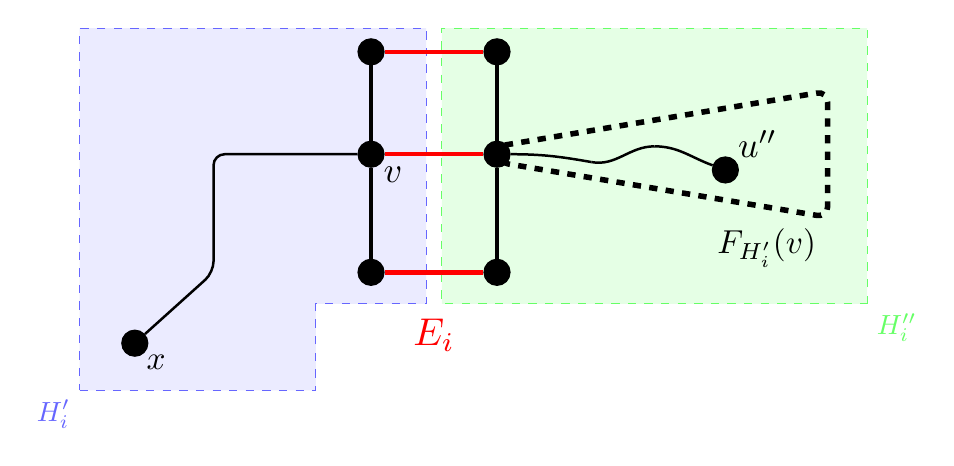
\begin{tikzpicture}

% AREAS %%%%%%%%%%%%%%%%%%%%%%%%%%%%%%%%%%%%%%%%%%%%%%%%%%%%%%%%%%%%%%%%%%

\draw [dashed, color = white!40!blue, fill = white!92!blue] (0,1.0) -- (3.0,1.0) -- (3.0,2.1) -- (4.4,2.1) -- (4.4,5.6) -- (0,5.6) -- (0,1.0) node[below left] {$H_i'$};
\draw [dashed, color = white!40!green, fill = white!90!green] (10.0,2.1) -- (10.0,5.6) -- (4.6,5.6) -- (4.6,2.1) -- (10.0,2.1) node[below right] {$H_i''$};

% NODES %%%%%%%%%%%%%%%%%%%%%%%%%%%%%%%%%%%%%%%%%%%%%%%%%%%%%%%%%%%%%%%%%%

%\node[draw, circle, minimum height=0.2cm, minimum width=0.2cm, fill=black] (P11) at (1,1) {};
%\node[draw, circle, minimum height=0.2cm, minimum width=0.2cm, fill=black] (P12) at (1,2.5) {};
\node[draw, circle, minimum height=0.2cm, minimum width=0.2cm, fill=black] (P11) at (0.7,1.6) {};
\draw (P11) node[below right,scale =1.2] {$x$};
%\draw[line width = 0.9pt,out=-10,in=180] (6.5,3.9)to(7.3,4.1);
%\draw[line width = 0.9pt,out=0,in=160] (7.3,4.1)to(P4);

\node[draw, circle, minimum height=0.2cm, minimum width=0.2cm, fill=black] (P22) at (3.7,2.5) {};
\node[draw, circle, minimum height=0.2cm, minimum width=0.2cm, fill=black] (P23) at (3.7,4) {};
\draw (P23) node[below right,scale = 1.3] {$v$};
\node[draw, circle, minimum height=0.2cm, minimum width=0.2cm, fill=black] (P24) at (3.7,5.3) {};

\node[draw, circle, minimum height=0.2cm, minimum width=0.2cm, fill=black] (P32) at (5.3,2.5) {};
\node[draw, circle, minimum height=0.2cm, minimum width=0.2cm, fill=black] (P33) at (5.3,4) {};
\draw [rounded corners, line width = 2pt, dashed] (5.3,4.1) -- (5.3,3.9) -- (9.5,3.2) -- (9.5,4.8) -- (5.3,4.1);
\draw (9.5,3.2) node[below left,scale =1.2] {$F_{H_i'}(v)$};
\node[draw, circle, minimum height=0.2cm, minimum width=0.2cm, fill=black] (P34) at (5.3,5.3) {};

\node[draw, circle, minimum height=0.2cm, minimum width=0.2cm, fill=black] (P4) at (8.2,3.8) {};
\draw (P4) node[above right,scale = 1.3] {$u''$};
\draw[line width = 0.9pt,out=0,in=170] (P33)to(6.5,3.9);
\draw[line width = 0.9pt,out=-10,in=180] (6.5,3.9)to(7.3,4.1);
\draw[line width = 0.9pt,out=0,in=160] (7.3,4.1)to(P4);

\draw[rounded corners, line width = 0.9pt] (P23) -- (1.7,4) -- (1.7,2.5) -- (P11);


% LINKS %%%%%%%%%%%%%%%%%%%%%%%%%%%%%%%%%%%%%%%%%%%%%%%%%%%%%%%%%%%%%%%%%%

\draw[line width = 1.6pt, color = red] (P22) -- (P32);
\draw[line width = 1.6pt, color = red] (P23) -- (P33);
\draw[line width = 1.6pt, color=red] (P24) -- (P34);

\draw[line width = 1.4pt] (P22) -- (P23);
\draw[line width = 1.4pt] (P32) -- (P33);
\draw[line width = 1.4pt] (P23) -- (P24);
\draw[line width = 1.4pt] (P33) -- (P34);


% ETIQUETTES

\node[scale=1.4, color = red] at (4.5,1.7) {$E_i$};

\end{tikzpicture}}
\caption{The largest weighted distance from $u'' \in H_i''$ to some vertex in $H_i'$ is given by the (unweighted) distance from $u''$ to its gate $v = g_{H_i'}(u'')$ in addition with the weighted eccentricity of $v$: $\wecc{v}{(H_i',\omega)} = d(v,x)$.}
\label{fig:fibers}
\end{figure}

One can retrieve at this moment the weighted eccentricity of $u' \in H_i'$ (resp. $u'' \in H_i''$ with the same arguments). Indeed, the farthest vertex from $u'$ (in the weighted sense) is either in $H_i'$ or in $H_i''$. If it belongs to $H_i'$, as this halfspace is convex, the weighted eccentricity of $u'$ is its label $\wecc{u'}{(H_i',\omega)}$. Else, as $H_i''$ is gated, for any vertex $v'' \in H_i''$, there is a shortest path from $u'$ to $v''$ passing through the $H_i''$-gate $g(u')$. Conversely, any shortest path induced in $H_i''$ from $g(u')$ to some $v''$, concatenated with a shortest $(u',g(u'))$-path, produces a shortest $(u',v'')$-path, since $d(u',g(u')) + d(g(u'),v'') = d(u',v'')$
. Hence, the weighted eccentricity of $u'$ can be decomposed as the sum of $d(u',g(u'))$ (distance to the gate) with the weighted eccentricity of $g(u')$ in $H_i''$. 
Formally, $$\wecc{u'}{(G,\omega)} = \max \left\{\wecc{u'}{(H_i',\omega)}, ~d(u',g(u')) + \wecc{g(u')}{(H_i'',\omega)}\right\}.$$ 
Figure~\ref{fig:fibers} illustrates this formula with a vertex $u'' \in H_i''$ instead of $u' \in H_i'$.
%: $$\ecc_G^+(u'') = \max\{\ecc_{H_i''}^+(u''), d(u'',g(u'')) + \ecc_{H_i'}^+(g(u''))\}.$$

The whole procedure, consisting first in computing the gates $g(u)$ and second in applying the latter formula, takes linear time $O(m)$.
\end{proof}

When our input graph $G$ has a balanced $\Theta$-class $E_i$, one can recursively compute the weighted eccentricities of the two induced halfspaces $G[H_i']$ and $G[H_i'']$ and then retrieve the weighted eccentricities of $G$ with an extra linear time. With some ``ideal'' instance, we could always find such a balanced $\Theta$-class and use this recursive scheme until falling into the trivial case of a single weighted vertex. Observe that, with such a utopian situation, the total running time would be quasilinear: the depth of the recursive tree is poly-logarithmic thanks to Lemma~\ref{le:log_decrease}. Indeed, fixing $s_0=n=\vert V(G) \vert$ and $\lambda  = 2$, value $s_n$ gives an upper bound of the number of vertices remaining in each branch of the recursive tree after $n$ calls. 

Nevertheless, we might find at some moment an induced subgraph of $G$ which has no balanced $\Theta$-class, in other words which belongs to $\ulog$. Obviously, even the input $G$ could belong to this family. As a conclusion of this section, we observe that, to pursue the description of our recursive algorithm, we need to focus on the case of weighted median graphs which admit only unbalanced $\Theta$-classes.

\section{Computation of eccentricities on median graphs without balanced $\Theta$-classes} \label{sec:unbalanced}

The study of median graphs with only unbalanced $\Theta$-classes is of interest since, as we prove it now, the existence of quasilinear-time algorithm finding all weighted eccentricities for the subfamily $\ulog$ of median graphs would imply the same result for the whole family of median graphs. From now on, we fix $(G,\omega) \in \ulog$. Notation $G$ naturally refers to the same graph without any weight consideration.

\PB{gérer les cas $G$ et $(G,\omega)$}

\subsection{Notation and preliminaries}

We pursue now with notations concerning $\Theta$-classes. As all $\Theta$-classes $E_i$ of $G \in \ulog$ are unbalanced, all of them admit both a minority halfspace denoted from now on by $H_i'$ (the halfspace with the smaller size), and a majority halfspace denoted by $H_i''$. From Definition~\ref{def:balanced}, we have $\vert H_i' \vert \le \frac{n}{2\log(n)}$ with $n = \vert V(G) \vert$. 

No graph of $\ulog$ contains an egalitarian halfspace since all its $\Theta$-classes are unbalanced. Consequently, these graphs admit a unique median vertex.

\begin{lemma}[Unique median vertex in $G\in \mathcal{U}_f$]
For any $G\in \mathcal{U}_f$ where $f(n) \ge 2$ for any integer $n \ge 2$, there exists a unique vertex $v_0$ such that, for any $\Theta$-class $E_i$ this vertex $v_0$ belongs to the majority halfspace of $E_i$.
\end{lemma}

\begin{proof}
From Lemma~\ref{le:majority}, the median set of a graph $G \in \mathcal{U}_f$ is the intersection of all majority halfspaces. Moreover, there exists $u,v \in V(G)$ such that $\med(G) = I(u,v)$. Assume that $u\neq v$. As $\med(G)$ is connected, consider two adjacent vertices $x,y \in \med(G)$ and let $xy \in E_i$. The $\Theta$-class $E_i$ admits two egalitarian halfspaces since, otherwise, either $x$ or $y$ would not be a median vertex. We have a contradiction as $E_i$ is clearly balanced.
\end{proof}

From now on, this unique median vertex $v_0$  will be taken as the basis of the orientation of $G$. We define $L(G)$ as a ladder set $L_{v_0,\umax}$ between $v_0$ and one farthest-to-$v_0$ vertex $\umax$.

\begin{definition}
Let $\umax$ be a vertex such that $d_{\omega}(v_0,\umax) = \wecc{v_0}{(G,\omega)}$. We denote by $L(G)$ the \textit{wide ladder} of $G$, which is the POF containing the $\Theta$-classes $E_i$ adjacent to $v_0$ such that $\umax$ belongs to their minority halfspace, {\em i.e.} $\umax \in H_i'$. Formally, $L(G) = L_{v_0,\umax}$ and $\ell = \vert L(G) \vert$ is its size.
\label{def:wide_ladder}
\end{definition}

In order to simplify our notation, we modify the indices of the $\Theta$-classes such that: $$L(G) = \{E_1,E_2,\ldots,E_{\ell}\}.$$ Observe that this change has no impact on the previous results since the indices of $\Theta$-classes were not considered yet.

Our technique to handle median graphs without balanced $\Theta$-classes relies on the following crucial observation. All vertices $v$ of $G$ such that $L_{v_0,v} \cap L(G) = \emptyset$ form, due to the unbalancedness of the $\Theta$-classes, a large set of vertices. Moreover, we can directly deduce their weighted eccentricity since $u$ is their extremal vertex. As a consequence, the eccentricity of at least half of the vertices of the graph are already known. We will explain how to handle the remaining vertices afterwards, in Section~\ref{subsec:slices}.

\begin{lemma}
Let $G \in \ulog$ and $v_0$ its median vertex. Any vertex $v$ such that $L_{v_0,v} \cap L(G) = \emptyset$ has a weighted eccentricity $\wecc{v}{(G,\omega)} = d(v,v_0) + d_{\omega}(v_0,\umax)$.
\label{le:ecc_large}
\end{lemma}
\begin{proof}
We show that $v_0 \in I(v,\umax)$. Let $P$ be a $(v,\umax)$-path consisting in the concatenation of a shortest $(v,v_0)$-path (denoted by $Q$) with a shortest $(v_0,\umax)$-path (denoted by $R$). It suffices to show that $P$ is made up of edges belonging to pairwise different $\Theta$-classes (Lemma~\ref{le:signature}). Assume by contradiction that there exists a $\Theta$-class $E_j \in I(v_0,v) \cap I(v_0,\umax)$ and that there is no other $\Theta$-class $E_k \in I(v_0,v) \cap I(v_0,\umax)$ such that:
\begin{itemize}
\item the edge of $E_k$ on path $Q$ is closer to $v_0$ than the edge of $E_j$ on $Q$,
\item the edge of $E_k$ on path $R$ is closer to $v_0$ than the edge of $E_j$ on $R$.
\end{itemize}
In brief, if we assume $I(v_0,v) \cap I(v_0,\umax)$ nonempty, we fix $E_j$ as a $\Theta$-class of this set which is minimal by distance towards the median vertex $v_0$. Such a minimal class necessarily exists.

By definition of $E_j$, there is no $\Theta$-class that appears twice in the path $P_j$, defined as the section of $P$ containing $v_0$ obtained after removing edges of $E_j$. Hence, $P_j$ is a shortest path. Moreover, its endpoints both belong to the same boundary $\partial H_j''$ of $E_j$. As $\partial H_j''$ is convex (Lemma~\ref{le:boundaries}) and $v_0 \in P_j$, then $v_0 \in \partial H_j''$. This yields a contradiction since $E_j$ is adjacent to $v_0$ and should be part of $L(G)$.
\end{proof}

\begin{definition}[Large sets]
We define recursively a finite sequence $\left(G_i\right)_{0\le i\le \ell}$ of induced subgraphs of $G$ called {\em large sets}. Let $G_0 = G$ and, for any integer $0\le i\le \ell - 1$,
$$G_{i+1} = G_i \setminus H_{i+1}'.$$
In other words, $G_{i+1}$ is incrementally obtained from $G_i$ by removing all vertices in the minority halfspace of $E_{i+1} \in L(G)$.
\label{def:large_sets}
\end{definition}

A first trivial remark is that the number of vertices of the graphs of the sequence is decreasing: $\vert V(G_{i+1}) \vert \le \vert V(G_i) \vert$. A second fact is that each $G_i$ is a gated subgraph of $G$.

\begin{lemma}
For each $0\le i\le \ell$, $G_i$ is a gated subgraph of $G$.
\label{le:gated_large}
\end{lemma}
\begin{proof}
We proceed by induction. Obviously, as the base case, $G_0 = G$ is trivially gated. 

We assume that $G_i$ is a gated subgraph of $G$: $V(G_i)$ is gated in $G$. Moreover, the halfspace $H_{i+1}''$ is also gated in $G$ (Lemma~\ref{le:halfspaces}). As we know from Definition~\ref{def:large_sets}, $V(G_{i+1}) = V(G_i) \setminus H_{i+1}' = V(G_i) \cap H_{i+1}''$. The intersection of two gated sets is gated (Lemma~\ref{le:intersection}). Hence, $V(G_{i+1})$ is gated and our induction step holds.
\end{proof}

In fact, we can rewrite, for any $1\le i\le \ell$, the definition of $G_i$ as the following one:
\begin{equation}
G_i = G[H_1'' \cap H_2'' \cap \ldots \cap H_i''].
\label{eq:large_sets}
\end{equation}

As all large sets $G_i$ are gated subgraphs of $G$, large sets are median graphs. So, they admit $\Theta$-classes which can in fact be retrieved from the $\Theta$-classes of the original graph $G$.

\begin{lemma}[$\Theta$-classes of isometric subgraphs~\cite{BeDuHa22}]
Let $G$ be a median graph. If $H$ is an isometric subgraph of $G$, then the $\Theta$-classes of $H$ are exactly the nonempty subsets among $E_i \cap E(H)$, for $E_i \in \mathcal{E}(G)$.
\label{le:isometric}
\end{lemma}

Since gated subgraphs are also isometric (the converse is false), then the $\Theta$-classes of $G_i$ are inherited from the $\Theta$-classes of $G$. 

We define \textit{slices} as the subgraphs withdrawn from each transition between $G_i$ and $G_{i+1}$.

\begin{definition}[Slices]
We define a finite sequence $(S_i)_{0\le i\le \ell - 1}$ of graphs called {\em slices}:
$$S_i = G_i \setminus V(G_{i+1}).$$
The vertex set of $G_i$ can be thus bi-partitioned with $S_i$ and $V(G_{i+1})$.
\label{def:corner}
\end{definition}

\PB{dessin slices et large sets}

Slices $S_i$ can be rewritten as the intersection of the minority halfspace $H_{i+1}'$ with the current vertex set $V(G_i)$: $S_i = G_i[H_{i+1}']$. In fact,
\begin{equation}
S_i = G\left[H_{i+1}' \setminus \left(H_1'\cup H_2'\cup \ldots H_i'\right)\right].
\label{eq:slices}
\end{equation}

\begin{lemma}
For each $0\le i\le \ell-1$, $S_i$ is a gated subgraph of $G$
\label{le:gated_slices}
\end{lemma}
\begin{proof}
Graph $G_i$ is gated subgraph of $G$ (Lemma~\ref{le:gated_large}). Consequently, $S_i$ is gated since it is the intersection between $H_{i+1}'$ and $V(G_i)$ (Lemma~\ref{le:intersection}).
\end{proof}

Slices are pairwise disjoint. In terms of cardinality, slices are thus small, $\vert V(S_i) \vert \le \vert H_{i+1}' \vert \le \frac{n}{2\log(n)}$, while even the last large set $G_{\ell}$ contains at least half of the vertices.

\begin{lemma}[Cardinality of large sets]
For any $0\le i\le \ell$, $\vert V(G_i) \vert \ge n(1-\frac{i}{2\log(n)})$.
\label{le:card_slices}
\end{lemma}
\begin{proof}
By induction: $i=0$ trivially holds. The large set $G_{i+1}$ corresponds to $G_i$ after withdrawing the slice $S_i$, which contains at most $\frac{n}{2\log n}$ vertices. Therefore, $$\vert V(G_{i+1}) \vert \ge \vert V(G_i)\vert - \frac{n}{2\log n} = n\left(1-\frac{i}{2\log(n)}\right) - \frac{n}{2\log n} = n\left(1-\frac{i+1}{2\log(n)}\right).$$
We obtain the announced inequality for all integers $0\le i\le \ell$.
\end{proof}

Indeed, as $\ell \le d\le \log n$, we have $\vert V(G_{\ell})\vert \ge  n(1-\frac{\ell}{2\log(n)}) \ge \frac{n}{2}$. From Equation~\eqref{eq:large_sets}, set $V(G_{\ell})$ contains exactly the vertices which does not belong to any $H_1',\ldots H_{\ell}'$, in other words whose ladder set has no intersection with $L(G)$. As stated in Lemma~\ref{le:ecc_large}, the weighted eccentricities of all vertices $v$ of $V(G_{\ell})$ can be directly deduced. On the other hand, any vertex $v$ with a ladder set $L_{v_0,v}$ intersecting $L(G)$ belongs to one of the slices $S_0,\ldots,S_{\ell-1}$ (Equation~\eqref{eq:slices}).

\subsection{Peeling the slices} \label{subsec:slices}

We show that, assuming we know all the weighted eccentricities on slices, which are small-sized induced subgraphs of the input graph $(G,\omega) \in \ulog$, we can deduce all weighted eccentricities of $G$. We begin with a description of how to modify weights on slices so that our recursive calls will enable us to retrieve all eccentricities.

\begin{definition}
Let $(G,\omega) \in \ulog$ and an integer $0\le i\le \ell-1$. The weight function $\omega_i^*$ on slice $S_i$ is defined as:
\begin{itemize}
\item for any $x \in \partial H_{i+1}' \cap V(G_i)$, $\omega_i^*(x)$ is equal to 
%the maximum between $\omega(x)$ and 
the maximum distance $d_{\omega}(x,z)$ where $z$ belongs to the fiber $F_{H_{i+1}'}(x)$ of $G_i$.\footnote{Here, we abuse notation: $H_{i+1}'$ refers to the intersection of $V(G_i)$ with $H_{i+1}'$, which is a halfspace of the $\Theta$-class $E_{i+1} \cap E(G_i)$ (Lemma~\ref{le:isometric}).}
\item for any $y \in V(G_i) \setminus \partial H_{i+1}'$, $\omega_i^*(y) = \omega(y)$.
\end{itemize}
\label{def:weights_slices}
\end{definition}

We state now a theorem which introduce our recursive process to compute the weighted eccentricities of $(G,\omega) \in \ulog$. As we already observed it, the eccentricity of the vertices of the large set $G_{\ell}$ are already known. Therefore, we focus on computing the eccentricities of the vertices of the slices. 

We define a labeling $\mathcal{B}_i$, for any $0\le i\le \ell-1$ on the vertices of $G_{i}$. This labeling gives:
\begin{itemize}
\item for any vertex $v \in V(G_{\ell})$, the maximum distance $d_{\omega}(v,z)$, where $z$ belongs to some slice $S_i \cup S_{i+1} \cup \ldots \cup S_{\ell - 1}$,
\item for any vertex $x \in S_i \cup S_{i+1} \cup \ldots \cup S_{\ell - 1}$, its weighted eccentricity on the graph $(G_i,\omega)$.
\end{itemize}

The label of $\mathcal{B}_i$ for some vertex $u \in G_i$ is denoted by $\beta_i(u)$. Observe that labeling $\mathcal{B}_0$ would allow us to determine all eccentricities of $(G,\omega)$: for vertices in the slices, the labels give their eccentricity while for vertices in $G_{\ell}$, we use Lemma~\ref{le:ecc_large}. 

Our proposition is the following. Assume that we already computed some labeling $\mathcal{B}_{i+1}$ and our intention is to obtain $\mathcal{B}_i$. Our idea to achieve this recursive step consists in launching two recursive calls, in order to compute the weighted eccentricities on graph $S_i$ but with two different weight functions $\omega$ and $\omega_i^*$. We prove that given labeling $\mathcal{B}_{i+1}$ and the results of these calls, we can retrieve labeling $\mathcal{B}_{i}$.

\begin{theorem}
Let $0\le i\le \ell-1$. Assume that the following values are known:
\begin{itemize}
\item all weighted eccentricities of $(S_i,\omega)$,
\item all weighted eccentricities of $(S_i,\omega_i^*)$,
\item all labels of $\mathcal{B}_{i+1}$.
\end{itemize}
One can compute in linear time $O(\vert E(G_i)\vert)$ all labels of $\mathcal{B}_{i}$.
\end{theorem}

\subsection{Summary and analysis for the eccentricities computation}

\begin{theorem}
Let $G \in \ulog$. Assume that $L = \{E_1,\ldots,E_r\}$ and that the eccentricities \ldots \PB{theoreme final pour les unbalanced, même forme que le theoreme final de 2.2}
\end{theorem}

\section{Distance profiles in diameter-bounded median graphs}

Let $G=(V,E)$ be a median graph with $n$ vertices, and let $D \ge 0$ to be fixed later in the proof.

\subsection{Reduction to median graphs with low diameter}

Let us recall the following results from our previous paper:

\begin{lemma}
    Let $G=(V,E)$ be an $n$-vertex median graph, let $E_1,E_2,\ldots,E_q$ be some of its $\Theta$-classes, and let $G_1,G_2,\ldots,G_p$ denote its isometric subgraphs obtained from the removal of all $\Theta$-classes $E_j$ with $1 \le j \le q$. If for every $i$ such that $1 \le i \le p$, the eccentricities of $G_i$ can be computed in $\Tilde{O}(T(n_i))$ time, where $n_i := |V(G_i)|$, then we can compute all eccentricities of $G$ in $\Tilde{O}\left(\sum_{i=1}^pT(n_i) + qn\right)$ time.
\end{lemma}

\begin{corollary}
    Let $G=(V,E)$ be an $n$-vertex median graph, and, for any $D \ge 0$, let $G_1,G_2,\ldots,G_p$ denote its isometric subgraphs obtained from the removal of all $\Theta$-classes with at least $D$ edges. If for every $i$ such that $1 \le i \le p$, the eccentricities of $G_i$ can be computed in $\Tilde{O}(T(n_i))$ time, where $n_i := |V(G_i)|$, then we can compute all eccentricities of $G$ in $\Tilde{O}\left(\sum_{i=1}^pT(n_i) + \frac{n^2}D\right)$ time.
\end{corollary}

In what follows, we may only consider median graphs such that every $\Theta$-class contains at most $D$ edges.
We prove the following new decomposition scheme for such median graphs:

\begin{lemma}
    Let $G=(V,E)$ be an $n$-vertex median graph such that every $\Theta$-class contains at most $D$ edges.
    There exists a subset of $\Theta$-classes $E_1,E_2,\ldots,E_q$ such that $q = \Tilde{O}(n/D)$, and every of the isometric subgraphs $G_1,G_2,\ldots,G_p$ obtained from the removal of all these $\Theta$-classes has diameter in $\Tilde{O}(D)$.
    Furthermore, the $\Theta$-classes $E_1,E_2,\ldots,E_q$ can be computed in $\Tilde{O}(n^2/D)$ time.
\end{lemma}

Note that the lemma holds with high probability for any random sample of $\Tilde{O}(n/D)$ $\Theta$-classes.
By contrast, our computation in what follows is deterministic.

\begin{proof}
Pick an arbitrary basepoint $u$ and execute a BFS from $u$.
Doing so, we compute its eccentricity $e(u)$.
If $e(u) \le D$, then $G$ has diameter at most $2D$, and so we are done.
Otherwise, let $v$ be a furthest from $u$ vertex.
Pick an arbitrary shortest $uv$-path, and select the edge $xy$ on it such that $d(x,v) > d(y,v) = D$ (such an edge must exist because we assume $d(u,v) = e(u) > D$).
Let $E_1$ be the $\Theta$-class of $xy$.
By removing $E_1$, we get isometric subgraphs $H_1,G_1$ such that $u \in H_1$ and $v \in G_1$.
We claim that $G_1$ has its diameter in ${O}(D)$.
Indeed, let $w$ be an arbitrary vertex of $G_1$. By construction of $G_1$ we have $d(u,w) \ge d(u,E_1) + d(E_1,w)$.
Since $G$ is a median graph, the boundaries are connected, and so, $d(u,E_1) \ge d(u,y) - |E_1| \ge d(u,y) - D = e(u) - 2D$.
Furthermore, $d(u,w) \ge e(u)$, which implies $d(w,E_1) \le 2D$.
For every $w' \in G_1$, we get $d(w,w') \le d(w,E_1) + |E_1| + d(E_1,w') \le 2D + D + 2D = 5D$, thus proving the claim.
Finally, we apply the process recursively to $H_1$.
Since $G_1$ contains at least $D$ vertices, namely, those on a shortest $yv$-path, this above process can only result in at most $n/D$ subgraphs $G_1,G_2,\ldots,G_p$.
\end{proof}

\subsection{Computation of the distance vectors}

Hence, we are left with computing all eccentricities in a median graph $G=(V,E)$ of diameter at most $D$.
For that, we are considering a seemingly more difficult problem, presented next:
\begin{itemize}
    \item Every vertex $v$ is assigned a $(D+1)$-dimensional vector $\overrightarrow{\pi}_G(v)$;
    \item For every vertex $v$, we want to compute a $(D+1)$-dimensional vector $\overrightarrow{\delta_G}(v)$ such that for every $0 \le i \le D$, $\delta_G(v,i) = \sum_{j=0}^i\sum\{ \pi_G(u,j) : d(v,u) = i - j \}$.
\end{itemize}
Initially, for every vertex $v$ we set $\pi_G(v,0) = 1$ and $\pi_G(v,i) = 0$ for every $1 \le i \le D$.
Then, $\delta_G(v,i)$ counts for the number of vertices at distance $i$ from $v$.
In particular, we can compute its eccentricity $e(v)$ from $\overrightarrow{\delta}_G(v)$, using the straightforward relation $e(v) = \max\{ i : \delta_G(v,i) > 0\}$.

\begin{definition}
Let $H_1',H_1''$ be complementary halfspaces of median graph $G=(V,E)$ such that $H_1'$ is a peripheral halfspace.
For every vertex $v'$ of $H_1'$, let $\overrightarrow{\pi}_{H_1'}(v') := \overrightarrow{\pi}_G(v')$.
For every vertex $v''$ of $H_1''$, let $\overrightarrow{\pi}_{H_1''}(v'')$ be as follows:
\begin{enumerate}
    \item If $v''$ is not in the boundary, then $\overrightarrow{\pi}_{H_1''}(v'') = \overrightarrow{\pi}_G(v'')$;
    \item Otherwise, let $v'$ be the unique neighbor of $v''$ in $H_1'$, we have:
    $$\begin{cases}
        \pi_{H_1''}(v'',0) = \pi_G(v'',0) \\
        \pi_{H_1''}(v'',i) = \pi_G(v'',i) + \pi_G(v',i-1) \ \text{for every} \ 1 \le i \le D
    \end{cases}$$
\end{enumerate}
\end{definition}

The following relation is the cornerstone of our new algorithm:

\begin{lemma}
    Let $H_1',H_1''$ be complementary halfspaces of median graph $G=(V,E)$, with respect to some $\Theta$-class $E_1$, such that $H_1'$ is a peripheral halfspace.
    The following properties hold:
    \begin{enumerate}
        \item For every vertex $v''$ of $H_1''$, $\overrightarrow{\delta}_G(v'') = \overrightarrow{\delta}_{H_1''}(v'')$;
        \item For every vertex $v'$ of $H_1'$, with $v''$ its unique neighbor in $H_1''$:
        $$\begin{cases}
            \delta_G(v',0) = \delta_{H_1'}(v',0) = \pi_G(v',0) \\
            \delta_G(v',1) = \delta_{H_1'}(v',1) + \pi_G(v'',0) \\
            \delta_G(v',i) = \delta_{H_1'}(v',i) + \delta_{H_1''}(v'',i-1) - \delta_{H_1'}(v',i-2) \ \text{for every} \ 2 \le i \le D
        \end{cases}$$
    \end{enumerate}
\end{lemma}
\begin{proof}
Let $v''$ be an arbitrary vertex of $H_1''$. 
Clearly, $\delta_G(v'',0) = \pi_G(v'',0) = \pi_{H_1''}(v'',0) = \delta_{H_1''}(v'',0)$.
For every $1 \le i \le D$, we have:
\begin{flalign*}
    \delta_G(v'',i) =& \sum_{j=0}^i\sum\{\pi_G(u,j) : d(v'',u) = i-j\} \\
    =& \sum_{j=0}^i\sum\{\pi_G(u',j) : u' \in H_1', d(u',v'') = i-j\} + \sum_{j=0}^i\sum\{\pi_G(u'',j) : u'' \in H_1'', d(u'',v'') = i-j\} \\
    =& \sum_{j=0}^{i-1}\sum\{\pi_G(u',j) : u''u' \in E_1, d(u'',v'') = i-j-1\} + \sum_{j=0}^i\sum\{\pi_G(u'',j) : u'' \in H_1'', d(u'',v'') = i-j\} \\
    =& \sum_{j=1}^{i}\sum\{\pi_G(u',j-1) : u''u' \in E_1, d(u'',v'') = i-j\} + \sum_{j=0}^i\sum\{\pi_G(u'',j) : u'' \in H_1'', d(u'',v'') = i-j\} \\
    =& \sum\{ \pi_G(u'',0) : u'' \in H_1'', \ d(u'',v'')=i\} + \sum_{j=1}^i\sum\{\pi_G(u'',j) : u'' \in H_1'' \setminus \partial H_1'', \ d(u'',v'') = i-j\} \\
    &+ \sum_{j=1}^i\sum\{\pi_G(u'',j)+\pi_G(u',j-1) : u''u' \in E_1, \ d(u'',v'') = i-j\}\\
    =& \sum_{j=0}^i\sum\{\pi_{H_1''}(u'',j) : u'' \in H_1'', \ d(u'',v'')=i-j\} \\
    =& \delta_{H_1''}(v'',i)
\end{flalign*}
Now, let $v'$ be an arbitrary vertex of $H_1'$, with $v''$ its unique neighbor in $H_1''$.
Again, we clearly have $\delta_G(v',0) = \pi_G(v',0) = \pi_{H_1'}(v,0) = \delta_{H_1'}(v,0)$.
Since $v''$ is the unique neighbor of $v'$ in $H_1''$, and $\overrightarrow{\pi}_{H_1'}$ is the restriction of $\overrightarrow{\pi}_G$ to $H_1'$, we also have $\delta_G(v',1) = \delta_{H_1'}(v',1) + \pi_G(v'',0)$.
Then, for every $2 \le i \le D$:
\begin{flalign*}
    \delta_G(v',i) &= \sum_{j=0}^i\sum\{\pi_G(u,j) : d(u,v') = i-j\} \\
    &= \sum_{j=0}^i\sum\{\pi_G(u',j) : u' \in H_1', \ d(u',v') = i-j\} + \sum_{j=0}^i\sum\{\pi_G(u'',j) : u' \in H_1'', \ d(u'',v') = i-j\} \\
    &= \sum_{j=0}^i\sum\{\pi_{H_i'}(u',j) : u' \in H_1', \ d(u',v') = i-j\} + \sum_{j=0}^{i-1}\sum\{\pi_G(u'',j) : u' \in H_1'', \ d(u'',v'') = i-j-1\} \\
    &= \delta_{H_1'}(v',i) + \delta_G(v'',i-1) - \sum_{j=0}^{i-1}\sum\{\pi_G(u',j) : u' \in H_1', \ d(u',v'') = i-j-1\} \\
    &= \delta_{H_1'}(v',i) + \delta_{H_1''}(v'',i-1) - \sum_{j=0}^{i-2}\sum\{\pi_G(u',j) : u' \in H_1', \ d(u',v') = i-j-2\} \\
    &= \delta_{H_1'}(v',i) + \delta_{H_1''}(v'',i-1) - \sum_{j=0}^{i-2}\sum\{\pi_{H_1'}(u',j) : u' \in H_1', \ d(u',v') = i-j-2\} \\
    &= \delta_{H_1'}(v',i) + \delta_{H_1''}(v'',i-1) - \delta_{H_1'}(v',i-2)
\end{flalign*}
\end{proof}
By using the above lemma, we can solve our problem by traversing backward and forward a peeling ordering $E_1,E_2,\ldots,E_q$ of the $\Theta$-classes of $G$, and calling our algorithm recursively on vertex-disjoint subgraphs of $G$ representing the successive boundaries. The total cost, excluding recursive calls, is in ${O}(Dm')$, where $m'$ is the number of edges to process (an edge of $E_i$ is processed if it is still present in the subgraph $G_i$ obtained from the successive contractions of $E_1,E_2,\ldots,E_{i-1}$). Since the subsets of edges processed at every recursion stage are pairwise disjoint, the final runtime is in ${O}(Dm) = \Tilde{O}(Dn)$.

\smallskip
Finally, the following result is obtained by setting $D = \sqrt{n}$:
\begin{theorem}
    We can compute all eccentricities in a median graph in $\Tilde{O}(n^{3/2})$ time.
\end{theorem}

\subsection{Comments (not visible)}

\begin{comment}
\iffalse
Consider the following input:
\begin{itemize}
    \item $G=(V,E)$ is a median graph;
    \item ${\cal L}_E \subseteq N_{\ge 1}$ is a subset of different labels for the $\Theta$-classes of $G$;
    \item Every vertex $v$ of $G$ is mapped to some subset $L(v) \subseteq {\cal L}_V \subseteq N_{\ge 1}$, such that ${\cal L}_V \cap {\cal L}_E = \emptyset$.
    Furthermore, there is a local mapping $\pi_v : L(v) \mapsto \mathbb{N}_{\ge 0}$.
\end{itemize}
Intuitively, the label sets $L(v)$ represent additional $\Theta$-classes incident to $v$ in a median supergraph $G'$ of $G$.
Then, for every $j \in L(v)$, one of the two half-spaces $H_j'$ of $G' \setminus E_j$, the one not containing $V(G)$, got removed.
Intuitively, the value $\pi_v(j)$ equals the maximum distance between $v$ and the vertices of $H_j'$ whose $v$ is the gate in $G$.
We consider the problem of computing the following values, for every vertex $v$ of $G$:
$$\begin{cases}
    e(v,0) = \max\{ d(v,u) + \pi_u(j) : j \in L(u) \setminus L(v) \} \\
    e(v,j) = \max\{ d(v,u) + \pi_u(j) : u \neq v, j \in L(u)\}, \ \text{for} \ j \in L(v).
\end{cases}$$

%\section{OLD}

In what follows, let $G=(V,E)$ be a median graph equipped with an orientation with base vertex $v_0$.
Being given a total ordering $E_1,E_2,\ldots,E_q$ of its $\Theta$-classes, let us write $G_0 := G$ then for every $1 \leq i \leq q$ let $G_i$ be obtained from $G_{i-1}$ by keeping the halfspace of $G_i \setminus E_i$ containing base vertex $v_0$.
It is a peripheral peeling if, for every $1 \leq i \leq q$, $B_i := V(G_{i-1}) \setminus V(G_i)$ is a peripheral halfspace of $G_{i-1}$.
A peripheral peeling can be computed in linear time.

Every $G_i$ is a gated subgraph of $G$. For every $v \in V_i := V(G_i)$, let $\pi_i^{\downarrow}(v)$ be the maximum distance between $v$ and a vertex of $V \setminus V_i$ of which $v$ is the gate in $G_i$. Note that $\pi_0^{\downarrow}(v) = 0$ for every $v \in V_0 = V$. For every $v \in V_i$, if $v$ is incident to an edge $vv' \in E_{i-1}$ then $\pi_i^{\downarrow}(v) = \max\{\pi_{i-1}^{\downarrow}(v),1+\pi_{i-1}^{\downarrow}(v')\}$; otherwise, $\pi_{i}^{\downarrow}(v) = \pi_{i-1}^{\downarrow}(v')$. 

For every $1 \leq i \leq q$, let also $H_i$ be the halfspace of $G \setminus E_i$ such that $V_i \cap V(H_i) = \emptyset$. For every $u \in B_i$, we define $\pi_i^{\uparrow}(u)$ as the maximum distance between $u$ and a vertex of $V \setminus V(H_i)$ of which $u$ is the gate in $H_i$. For the unique $u \in B_q$, let $v_0$ be the unique vertex of $G_q$ (neighbour of $u$). We have $\pi_q^{\uparrow}(u) = 1 + \pi^{\downarrow}_{q-1}(v_0)$.

Let $G=(V,E)$ be a median graph.  
We compute a peeling order $E_1,E_2,\ldots E_q$ of its $\Theta$-classes.
By sequentially contracting the $\Theta$-classes in order, we obtain a sequence $G_0,G_1,\ldots G_q$ of convex subgraphs of $G$ such that $G_0 := G$ and $G_q$ is a singleton.
For each vertex $v \in V_i := V(G_i)$, let $w_i(v)$ be the maximum distance between $v$ and a vertex of $V \setminus V_i$ of which $v$ is the gate in $G_i$.
Observe that $w_0(v) = 0$.
Given the $\Theta$-class $E_i$ of which we contract the border, if $uu' \in E_i$ then $w_i(u') = \max\{w_{i-1}(u'),1+w_{i-1}(u)\}$. 

%\section{Diameter}

\bigskip

Let $u$ be an arbitrary basepoint and let $v$ maximize $d(u,v)$.
If $d(u,v) \leq D$ then, $diam(G) \leq 2D$.
Otherwise, let $xy$ be an edge on a shortest $uv$-path satisfying $d(v,x) = D < d(v,y)$, and let $E_i$ be its $\Theta$-class.
Let $H_i',H_i''$ be the corresponding halfspaces, and note that $u \in V(H_i'), \ v \in V(H_i'')$.
For every $w \in V(H_i'')$ let $w^*$ be its gate in $\partial H_i''$.
We have $d(u,w) = d(u,w^*) + d(w^*,w) \leq d(u,x) - |E_i| + d(w^*,w)$.
Since $d(u,v) = d(u,x) + d(x,v) \geq d(u,w)$, we get $d(w^*,w) \leq |E_i| + d(x,v) \leq D + |E_i|$.
In particular, $diam(H_i'') \leq 2(D + |E_i|) + |E_i| = 2D + 3|E_i|$

The process takes linear time. It removes at least $D$ vertices each step (namely, a shortest $vx$-path), and therefore, it can only be repeated at most ${O}(n/D)$ times.

Now consider a median graph of diameter at most $D$ and where each $\Theta$-class contains at most $D$ edges.
To compute the list of eccentricities, we solve the more general problem of computing the distance distribution, namely: for each vertex $v$ and integer $0 \leq i \leq D$, let $\delta(v,i) = \# \{ x \mid d(v,x) = i \}$. 
Let us solve an even more general problem. Let $w : V \to [D]^{[D]}$, where $[D] = \{0,1,\ldots,D\}$.
Then, we define $\delta_w(v,i) = \sum_{j=0}^i\sum\{ w(x)[j] \mid d(v,x) = i - j \}$.

For that, start from a peripheral halfspace $H$. 
Compute recursively on $H$.
Then, for every $v \in V(H)$, let $v^*$ be its gate.
We modify $w(v^*)$ so that, for every $i > 0$, $w(v^*)[i] := w(v^*)[i] + w(v)[i-1]$.
Then, we compute recursively on $G \setminus H$.
Doing so, all values $\delta_w(\cdot,\cdot)$ were correctly computed for $G \setminus H$.
For $v \in H$, let $\tilde{\delta}_w(v,\cdot)$ be computed in $H$.
Then,  $\delta_w(v,i) = ??$

\bigskip
Assume that every vertex has two vertex-weights, denoted $\pi,w$.
For every vertices $u$ and $v$, let $d_w(v,u) = d(v,u) + w(u)$. Note that it is not symmetric.
Let $e_w(v) = \max_u d_w(v,u)$.
Finally, let $p_w(v) = \sum\{\pi(u) \mid d_w(v,u) = e_w(v)\}$.
Our goal is to compute $(e_w(v),p_w(v))$ for every vertex $v$.

Consider $H_i'$ a peripheral halfspace.
For every $v \in H_i'$ let $v^*$ be its gate in $H_i''$.
Set $\tilde{w}(v^*) := \max\{w(v^*),1+w(v)\}$.
Let also: $$\tilde{\pi}(v^*) := \begin{cases}
\pi(v^*) \ \text{if} \ w(v^*) > w(v) + 1 \\
\pi(v) \ \text{if} \ w(v) + 1 > w(v^*) \\
\pi(v) + \pi(v^*) \ \text{otherwise.}
\end{cases}$$
We claim that $\tilde{e}(u) = e(u)$ and $\tilde{p}(u) = p(u)$ for every $u \in H_i''$.
Now, for $v \in H_i'$, compute $\bar{e}(v),\bar{p}(v)$ in $H_i'$.
Note that $e(v^*) \geq 1 + \bar{e}(v)$.
First assume $e(v^*) > 1 + \bar{e}(v)$.
Then, $e(v) = e(v^*)+1$ and $p(v) = p(v^*)$.
From now on, $e(v^*) = 1 + \bar{e}(v)$.
If $p(v^*) = \bar{p}(v)$ then, 

%\maketitle

In what follows, let $G=(V,E)$ be a cube-free median graph, let $c \in V$ be a centroid, and let $S = St(c)$ be the corresponding star.
Finally, for each $x \in S$, let $F(x)$ be its fiber.


\begin{lemma}
Let $u \in F(x)$ and $v \in F(y)$. If $F(x)$ and $F(y)$ are not separated then, $c \notin I(u,v)$.
\end{lemma}
\begin{proof}
Suppose by contradiction $c \in I(u,v)$. Since $x \in I(u,c)$ and $y \in I(v,c)$, there exists a shortest $uv$-path which contains $x,c,y$.
But either $xy \in E$ (if $F(x),F(y)$ are $1$-neighbouring) or there exists a $z \in N(c) \cap N(x) \cap N(y)$ (if $F(x),F(y)$ are $2$-neighbouring).
A contradiction.
\end{proof}

%\section{OLD}


Denote $e_G(v)$ the eccentricity of vertex $v$ in some graph $G$.
Our goal is to compute the eccentricities in a median graph.
For that, we start with a simple observation:

\begin{lemma}\label{lem:theta-class}
Let $E_i$ be a $\theta$-class of some median graoh $G$, let $H_i$ and $H_i'$ be the corresponding half-spaces, and let $\partial H_i, \partial H_i'$ be the boundaries.
For every $v_i \in V(H_i)$, let $u_i \in \partial H_i$ be its gate, and let $u_i' \in \partial H_i'$ be such that $u_iu_i' \in E_i$.
Then, $e_G(v_i) = \max\{e_{H_i}(v_i), d_{H_i}(u_i,v_i) + 1 + e_{H_i'}(u_i')\}$.
\end{lemma}


%\section{Other approach}

Let $G=(V,E)$ be a median graph of dimension $d$.
Then, $G$ has at most $2^dn$ hypercubes.
If every $\Theta$-class is selected independently at random with probability $p$, then a fixed hypercube is left intact with probability at most $(1-p)^d$.
Let $\alpha = 2(1-p)$. Then, we want:
$$ \alpha^d n = 1/2  $$
In other words, $\alpha = 1/(2n)^{\frac 1 d} = 2^{-\frac{1+\log{n}}{d}}$
\fi

\end{comment}

%Bibliographie
\bibliographystyle{plain}
\bibliography{median}

\end{document}
